% !TeX root = ../../paper.tex
\subsubsection{Vorsortieren}

Damit der Alpha-Beta Algorithmus, der in Kapitel~\ref{ch:alpha-beta-pruning} beschrieben wurde, bestmöglich wirken kann, müssen die aussichtsreichsten Züge zuerst durchsucht werden [\cite{Wiki2019}].
Es existieren verschiedenste Herangehensweisen, dies umzusetzen.
Da die möglichen Spielzüge in einem Suchgraphen abgebildet werden können und ein Schachcomputer für den allgemeinen Bedarf möglichst wenig Speicher benötigen sollte, bietet sich das \textit{Depth-First} Suchverfahren (zu dt. etwa \textit{Tiefensuche}) an.
Dabei werden zuerst tieferliegende Knoten ausgewertet, bevor benachbarte Knoten ausgewertet werden.
Das Depth-First Verfahren bietet den Vorteil, dass nur jeweils ein Pfad des Baumes im Speicher gehalten werden muss [\cite{Wiki2019b}].
Abbildung~\ref{fig:pre-sorting_depth-first-tree} zeigt eine beispielhafte Evaluierung eines Baumes nach dem Depth-First Verfahren.

\begin{figure}[H]
    \centering
    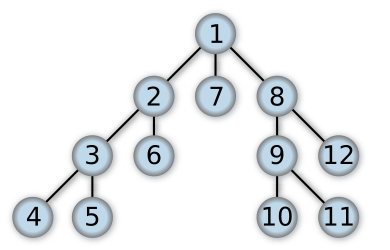
\includegraphics[width=0.6\textwidth]{images/theory/pre-sorting_depth-first-tree.png}
    \caption[Beispielhafter Depth-First Baum]{Beispielhafter Depth-First Baum [\cite{Wiki2019b}]}
    \label{fig:pre-sorting_depth-first-tree}
\end{figure}

\noindent Die Zahlen innerhalb der Knoten repräsentieren die Reihenfolge, in der die Knoten besucht werden.
Im Beispiel wird zuerst der Wurzelknoten betrachtet.
Von diesem ausgehend wir der am weitesten links befindliche Kindknoten evaluiert (markiert durch die Zahl 2).
Der nächstfolgende Knoten ist wiederum der am weitesten links befindliche Kindknoten, in der Abbildung markiert durch die Zahl 3.
Nachdem der Knoten mit der Zahl 4 evaluiert wurde, ist die maximale Tiefe für diesen Pfad erreicht, da der Knoten mit der Zahl 4 keine Kindknoten besitzt.
Aus diesem Grund wird eine Ebene höher beim Knoten mit der Zahl 3 geschaut, ob dieser noch weitere Kindknoten besitzt.
Da dies der Fall ist, werden jene weiteren Kindknoten evaluiert.
Im abgebildeten Beispiel betrifft dies ausschließlich den Knoten mit der Zahl 5.
Da weder Knoten 5 noch eine Ebene höher Knoten 3 weitere Kindknoten besitzen, wird wieder eine Ebene weiter oben geschaut.
Dieser Prozess wird solange fortgeführt, bis alle Knoten besucht wurden.

Weil ein Schachcomputer, der in einem Spiel gegen einen Menschen Einsatz findet, in einer für seinen Gegner vertretbaren Zeit antworten muss, werden Zeitmanagementstrategien benötigt.
Diese legen fest, in welcher Reihenfolge die möglichen Spielzüge ausgewerten werden, um die aussichtsreichsten Spielzüge möglichst am Anfang durchzurechnen.
Bei den Depth-First Suchverfahren hat sich das \textit{Iterative Deepening} (zu dt. etwa \textit{iterative Tiefensuche}) als grundlegende Zeitmanagementstrategie durchgesetzt.
Bei dieser Zeitmanagementstrategie werden alle möglichen Pfade eines Spielbaumes bis zu einer Tiefe von~1 ausgewertet.
Ist nach Abschluss der Auswertung die verfügbare Zeit des Spielzugs noch nicht abgelaufen, so wird die Suchtiefe um eins erhöht und eine weitere Evaluierungsphase beginnt [\cite{Wiki2019a}].
Abbildung~\ref{fig:pre-sorting_iterative-deepening} stellt diesen Vorgang grafisch an einem Beispiel dar.

\begin{figure}[H]
    \centering
    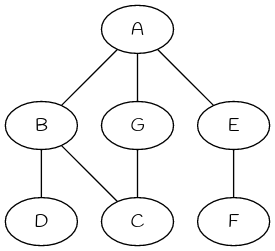
\includegraphics[width=0.6\textwidth]{images/theory/pre-sorting_iterative-deepening.png}
    \caption[Grafische Darstellung der Zeitmanagementstrategie Iterative Deepening]{Grafische Darstellung der Zeitmanagementstrategie Iterative Deepening}
    \label{fig:pre-sorting_iterative-deepening}
\end{figure}

\noindent Bei der folgenden beispielhafter Erläuterung des Iterative Deepening wird angenommen, dass die Knoten von links nach recht abgearbeitet werden.
Im ersten Durchlauf werden bei einer Tiefe von~1 nur die Knoten A B G und E evaluiert.
Somit sind dem Schachcomputer jetzt bereits alle möglichen Spielzüge bis zu einer Tiefe von eins bekannt, sodass er bei Abbruch des Spielzuges aufgrund der abgelaufenen Zeit bereits eine mögliche gute Entscheidung fällen kann.
Darstellung~\ref{eq:pre-sorting_iterative-deepening-example} zeigt die Reihenfolge der ausgewerteten Knoten für die Tiefen~2 und~3.

\begin{align} \label{eq:pre-sorting_iterative-deepening-example}
\begin{split}
    & \text{Tiefe 2: } A\ B\ D\ C\ G\ C\ E\ F\\
    & \text{Tiefe 3: } A\ B\ D\ C\ G\ G\ C\ B\ E\ F
\end{split}
\end{align}
